\chapter{Access point clustering}
%To enable collaborative channel allocation, it is
%important for every AP to know which APs it is collaborating with.
%One way to share information about who collaborates with who,
%is to let the access points group together. Information relevant for channel
%allocation can then be shared freely within the group, between APs.

%We will proceed by looking at some of the requirements for a group creation algorithm.
%It should work decentralized in a distributed fashion. Hence, not only does the APs have to
%be imposed group membership, but they also have to be able to create and definine
%meaningful groups on their own. Later we will propose an algorithm to create groups,
%and then evaluate computed groups based on the algorithm.


\section{Introduction}
While it at first sounds incredibly desirable to let the entire population of for instance New York's access points organize themselves in an optimal channel-plan,
at second thought the idea may prove to be a little ambitious. Being limited by the NP-complete nature of DSATUR or similar graph coloring algorithms
we have to set some reasonable constraints on the size of the \textit{collaborating group}. The amount of nodes that will collaborate on the problem of finding an optimal channel distribution
plan may not need to be very high.

Let us for a moment look at an ideal example: a city that only consists of small apartment buildings that are entirely isolated from interference produced in external networks.
How could we build a group in such a case? Turns out it is not that hard. Each access point would be able to collaborate with every other observable access point.
When computing channel distribution there would be no risk of surpassing the viable amount of nodes to compute the distribution for, as the group is limited to the apartment building. Sadly for us the world is not ideal,
and it is not impossible that every access point in New York can observe eachother through a transitive relation. This means the size of
the collaborating group would be vast and completely unviable.  

This does not mean that creating reasonably sized groups of access points is impossible, but it poses a more difficult challenge. 
We need to filter out redundant nodes to create an approximated version of the ideal example.

Having a picture of the typical cityscape in mind, we know that buildings are naturally
separated by streets, bridges, parks, and so on. Rural areas are similar, but networks are spaced more unevenly
and usually only affecting each other in one plane.

Remembering attenuation, we know that RF-interference is also a property of distance. 
These pieces of information tells us that RSSI readings between access points in two separated buildings should be lower than readings between access points in adjacent apartments.
What we will be looking at in the following chapter is how we can utilize the RSSI readings between access points to build a clustering algorithm that creates reasonable groups
of access points that discriminates between low-impact and high-impact nodes.  

%The should consist of APs that interfere with each other when their channels are overlapping, so that overlap can be avoided with a channel allocation algorithm run within the group. Not all APs in
%the connected group will necessarily be able to hear each other on the radio directly, but all nodes
%should be able to hear each other through a transitive relation (neighbour of a neighbour, etc.).

\section{Problem overview}
The main problem we are dealing with is finding a way for access points to group together in clusters that are geographically close to each other. This can either be solved with a centralized
coordinator or with a peer-to-peer distributed protocol. In this thesis we will be focusing on the distributed approach, but first we will take a look at the pros and cons of each approach, and
the work that has already been done on the field.
\subsection{Centralized model}
Let us briefly envision how a centralized model might look. As we want to propose a solution that works across private consumer networks as well as larger corporate networks,
we can not assume that all networks are under the same administrative domain. This is where the centralized approach is limited, and why it may not be ideal.

Just like the distributed version is, the centralized controller is also restricted by the NP-complete nature of all graph colouring algorithms.
To be able to create a channel plan which is as optimal as possible, it has to identify groups of nodes that impacts each other severely. 

The advantage of the centralized model is the ability to have the full picture of access points readily available. Let us assume the controller is placed at an ISP or a router manifacturer.
The controller could potentially know exactly where in the world the access points are placed. Creating groups would
be as simple as dividing within naturally separative geographical barriers like roads, streets and buildings. 

For a central controller to be able to identify APs that are near eachother and compute the optimal channel distribution, APs need to report their radio readings to the controller. 
The controller then needs to identify which of all the observed APs it can control, and which is not controllable and has to be treated as noise. There would be no requirement for
communication in between nodes, which reduces complexity a lot.  

A major drawback of the centralized approach is that nodes that are near eachother have to be under the same controller. If there are too many nodes around
that can not be controlled by the controller, all nearby access points would be treated as noise and regular channel allocation schemes would have to be applied.
Even though in there is a tendency for apartments in the same building to have the same ISP in Norway, there is no gurantee for that to always be the case.  

\subsection{Distributed approach}
Now that we have looked at how a centralized model might look, we can dive further into the main matter of the thesis. A simplistic way to portray the idea behind
the distributed approach is: nodes only depend on their own radio RSSI readings to be able to create groups. When the group is formed, all of its members can
compute a channel plan which is as optimal possible. In reality this idea has some major challenges that we have to overcome. Here are the most prominent ones: 
\begin{itemize}
	\item The communication channel. Nodes have to be able to communicate with eachother. The 802.11 standard describes no protocol for communication between access points that are not on the same extended service set. This communication would have to happen on the network layer, preferably over TCP. This communication channel would have to convey a messages that enables group creation,
		most likely a custom protocol. 
	\item The group creation itself. Based on only the RSSI-readings and the communication channel, nodes have to be able to organize themselves in a tight cluster of nodes that
		includes all nodes that impacts each other most severely. This problem essentially boils down to a clustering problem. This is the main issue we will
		try to find a reasonable solution for. 
	\item Node state. As all nodes have to compute a channel plan for the group, they all need to have the same consistent information about the members of the groups
		and every other node's RSSI-readings. 
	\item Channel plan computation. Even though the centralized approach would have a similar problem, it can be more difficult to solve in a distributed fashion, as 
		it is reasonable to assume that an access point has limited computational power. We will not discuss a solution for this in depth, as it is out of the scope
		of the thesis, but there are already a couple of algorithms that treat channel allocation as a graph colouring problem. 
\end{itemize}


\section{Computation assumptions and requirements}
Proceeding in the next chapters we will be looking at possible ways for nodes to organize themselves into groups in a peer-to-peer fashion.
The data we will be using is the data we fetched in chapter \ref{dataacc} and structured in the JSON format described. The data provides
a topology of nodes where all nodes have a list of neighbours that they can hear, with the appropriate RSSI-reading for how loud they can be heard.   
This is the only information the nodes are given, and based on the RSSI-values of their neighbours they should be able to organize themselves. 
To simplify the computation procedure and to reduce the workload for building the program we are going to to a number of assumptions. 

    \begin{enumerate}
    \item All APs visible on any AP's radio also runs the group creations algorithm. This is an assumption needed to be able to
	see how well the group performs in an optimal condition. It can be interesting to add rogue nodes that does not take part in group creation at a later point
	to see how well group creation works in a less optimal condition. 
    \item If a node has another node in its neighbour list (meaning that they can hear each other on their radio), it also knows how to directly contact the node (e.g. via TCP).
	 There is an underlying and working protocol that lets nodes communicate and exchange information about their RSSI-readings and group membership. 
    \item All nodes in a group are completely synchronous, and always have an equal image of the state of the group at a given time. 
    \end{enumerate}

\section{Proposing an algorithm}\label{algorithm}
With the definition of a connected group in place, and the assumptions and requirements accounted for, we can begin proposing an algorithm.

Henceforth we will for the sake of simplicity be referring to APs that are running the group algorithm as \textit{nodes}.

Each node begins by identifying itself as a member of a group that only contains itself. Let us call it group $a$. The node shares all of
its radio readings with the rest of the members in group $a$. Group $a$ looks at all the radio readings of every member, and picks the node with the highest dBm value
to contact. Of course in the beginning there is only one node in group $a$, so this node's radio readings alone will decide which group to merge with. 

The neighbour node that has the highest dBm value is in group $b$, and this is the most crucial node to collaborate with. Hence the group $a$ merges its own group together
with the group of neighbour $b$. This happens in the following way: the members of the two groups exchange information about all their member nodes and their radio readings.
The data is now identical for all the members of both groups, and they can make identical choices, hence they are now in the same group. 

If the number of members $n$ exceeds a predefined threshold $memberThresh$ after a merge, the group should begin kicking out members from the group, starting with the node
that influences the rest of the group the least. 

To prevent the group from oscillating between kicking out members and rejoining members, once it reaches
its maximum size it should be locked for further merges. 

\section{Program design}
The program is designed so that it can be modified to accomodate different algorithm types, while still keeping the basic framework untouched.
It is implemented in Python 3 \cite{Python3}, and is designed to run on the output from the data generation program. Seperating these programs is important,
as group computation should be fast operation, while the data generation (or fetching) is a slow process and should only be done once every time a new data set is required. 
A major design choice that had to be made early in the planning process  was whether or not the computation should be run in parallel or in sequence. 

If the program was implemeneted in a way that computation ran in parallel, it could assign one thread to each node, and let the nodes interact through an interface to one another. Thus simulating a
peer-to-peer protocol interface. Comparing with a sequential implementation, a parallel computation could arguably be a better representation of the real world,
as the nodes act independely of each other and the order of events is to some degree random.
It is exactly because of this chaotic nature of parallel computation that the program is designed to run in sequence.
The benefit of this is consistent and recreateable results which for needs outweighs the benefits of a parallel implementation. It also reduces the complexity of doing operations
on groups memberships since we don't get any race conditions. This particular point is also accounted for in the program assumptions, where we assume that all nodes have the exact same state.
It has to be said that given a perfect algorithm that always find the best division of groups, the resulting groups should end up being the same whether or not it is done sequentially or in 
parallel, but at this point we don't know what results to expect. 


The group framework consists of 3 classes with different responsibilities:
\begin{itemize}
	\item \textbf{Group}. An object of this class is an abstraction of all the nodes that belong to the same group. Because we have assumed that all nodes have equal
	information about group membership and RSSI-readings, we can store all the members of each group in a list and let the group object act as a unified entity on
	behalf of the entire group. All the interfaces and logic for forming groups is placed within this class. A method named \verb|iteration|
	has the responsibility of triggering the appropriate action based on the state of the group. For instance adding node, removing a node or merging the group
		with another. If an action was performed the method returns 1, else it returns 0. 

	\item \textbf{GroupCollection}. An object of this class should contain all the groups used in a simulation. Its main functional responsibility is looping through all the groups
	and calling the \verb|iteration| method once. This is done in the GroupCollection's \verb|iterate| method. It accumulates the amount of changes done in all the groups,
	by adding the return values of the Group object's \verb|iteration| method. It also handles the destruction of groups, and bootstrapping of newly created groups.

	\item \textbf{Simulation}. An object of this class handles the bootstrapping of groups, where all nodes (given in the input file) are parsed and
	put in their own grown group. Consequently at the beginning of each computation the amount of groups is equal to the amount of nodes.
	The Simulation class is also responsible for starting and stopping the simulation itself. After bootstrapping all the groups, the Simulation enters a loop
	where it calls the \verb|iterate| method in the GroupCollections object once every run. All the groups have converged and reached a steady state 
	once the amount of changes returned by the GroupCollection's \verb|iterate| method is equal to zero. The results are written to file.

\end{itemize}
\begin{algorithm}[H]
	\KwData{this text}
			\KwResult{how to write algorithm with \LaTeX2e }
			initialization\;
			\While{not at end of this document}{
				read current\;
			\eIf{understand}{
				go to next section\;
			current section becomes this one\;
		}{
			go back to the beginning of current section\;
		}
	}
			\caption{How to write algorithms}
\end{algorithm}

\section{Results}

\subsection{Uniformly distributed nodes}
We will look at how groups were created in different topology scenarios. 
All topologies presented in this section was created by the topology generation program,
but with different input parameters. Groups are distinguished by node color, where nodes
of the same color represents members of the same group. 
\subsubsection{Scenario 1}
Computed with 200 nodes with a maximum of 128 members in each group.

As can be seen in figure \ref{fig:200_128} the algorithm divides the nodes in two
sections. For clarity, a divisive line has been drawn around each group,
in case colors are not available.
When two major groups merged, the biggest groups surpasssed 128 members and began
kicking out members. The excess members formed the black group at the bottom. 

\begin{figure}
\center
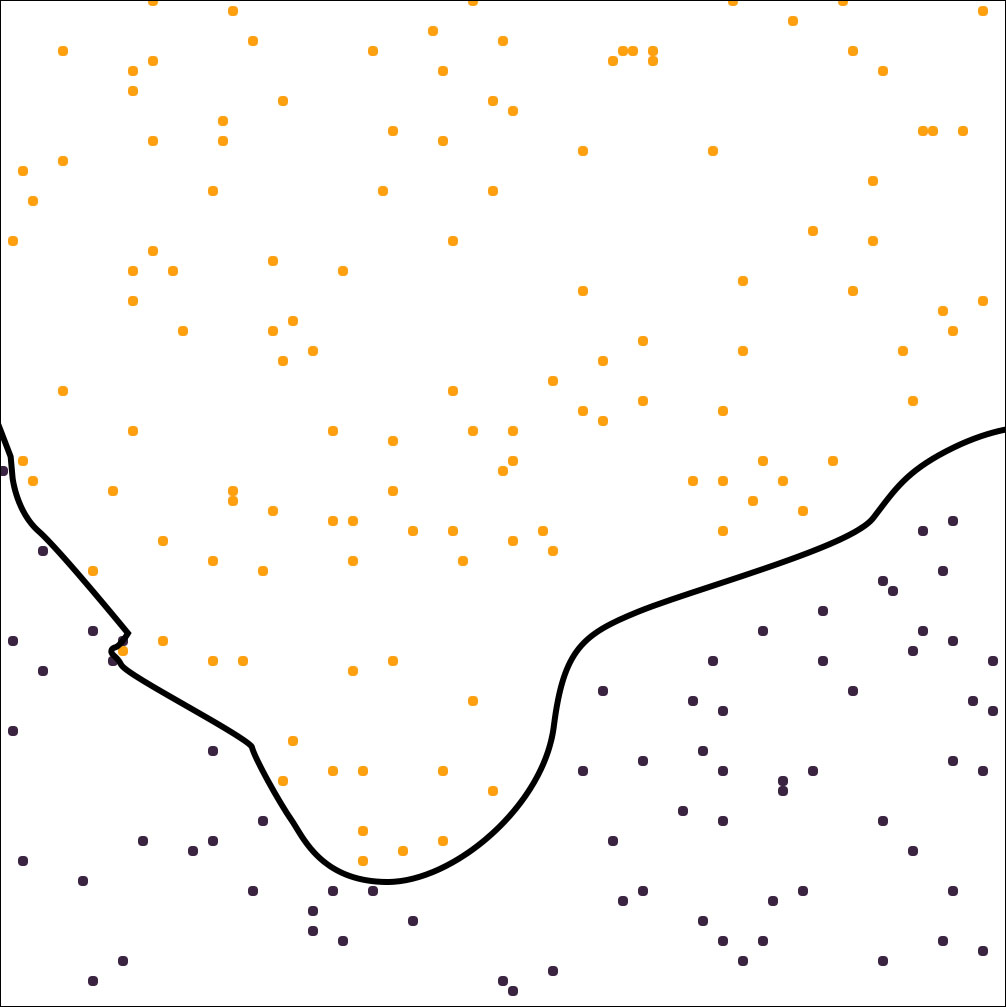
\includegraphics[scale=0.45]{Images/grouptest_1.jpg}
\caption{200 nodes, $memberThresh=128$, $size=200x200$}
\label{fig:200_128}
\end{figure}


\subsubsection{Scenario 2} \label{scen2}
Computed with 200 nodes with a maximum of 10 members in each group.

The result of this computation, seen in figure \ref{fig:200_10}, is a little less obvious.
The groups are again distinguished by different color, but for clarity we add a gray connecting
blob for nodes in the same group. Also blobs connected with a line are in the same group. 

It is worthy to take notice that one group is especially scattered around the graph.
At first eyesight, it looks like an algorithm deficiency, but the reason is quite simple:
when nodes are kicked out of a group during a merge, they will connet to other nodes
that belong in a group where $n$ has not yet reached $memberThresh$. When this have happened a couple of times, everyone has found a group except for the remaining few.
These are typically straggler nodes or smaller clusters separated from the others.
They are not big enough to reach the group $memberThresh$ on their own, so the merge with other
nodes that are in unmaxed groups. Thus, even though they have neighbours which
influence them more, they can only merge with nodes further away,
because that is the only unlocked group that remains.
\begin{figure}
\center
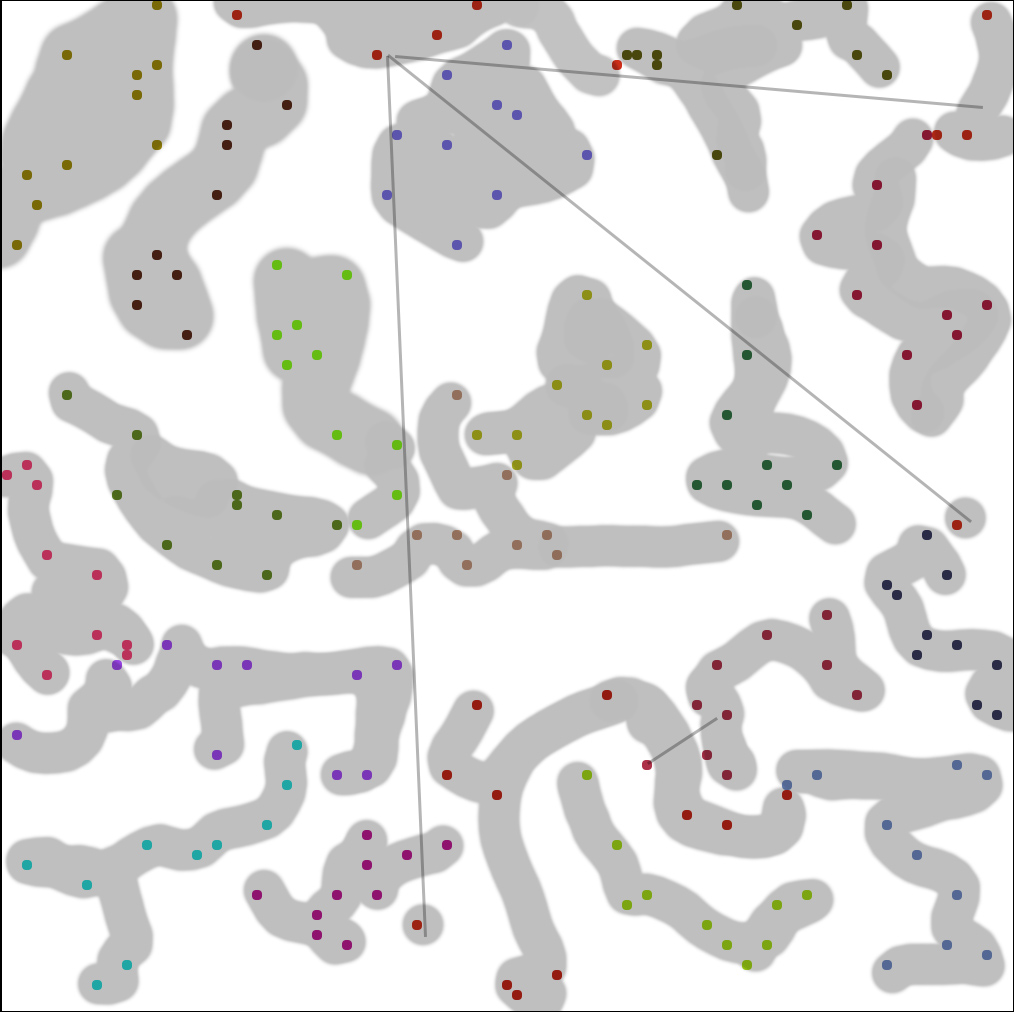
\includegraphics[scale=0.45]{Images/grouptest_2.jpg}
\caption{200 nodes, $memberThresh=10$, $size=200x200$}
\label{fig:200_10}
\end{figure}

\subsubsection{Scenario 3}
Computed with 5000 nodes, with a maximum for 64 members in each group. 

Figure \ref{fig:2000_64} shows the result of the computation. Because of the quantity
of nodes and the clear separation of groups, they are easily distinguished by color.
This topology is much denser than the others, and can vaguely resemble the density of highly populated areas.

We can clearly see that the overall tendency is that groups are formed
in concentrated areas of nodes. However, some groups are scattered, sometimes
all over the map. An example of a scattered group is highlighted
in figure \ref{fig:2000_64}. Its  member nodes has a thicker black line around them. 
\begin{figure}
\center
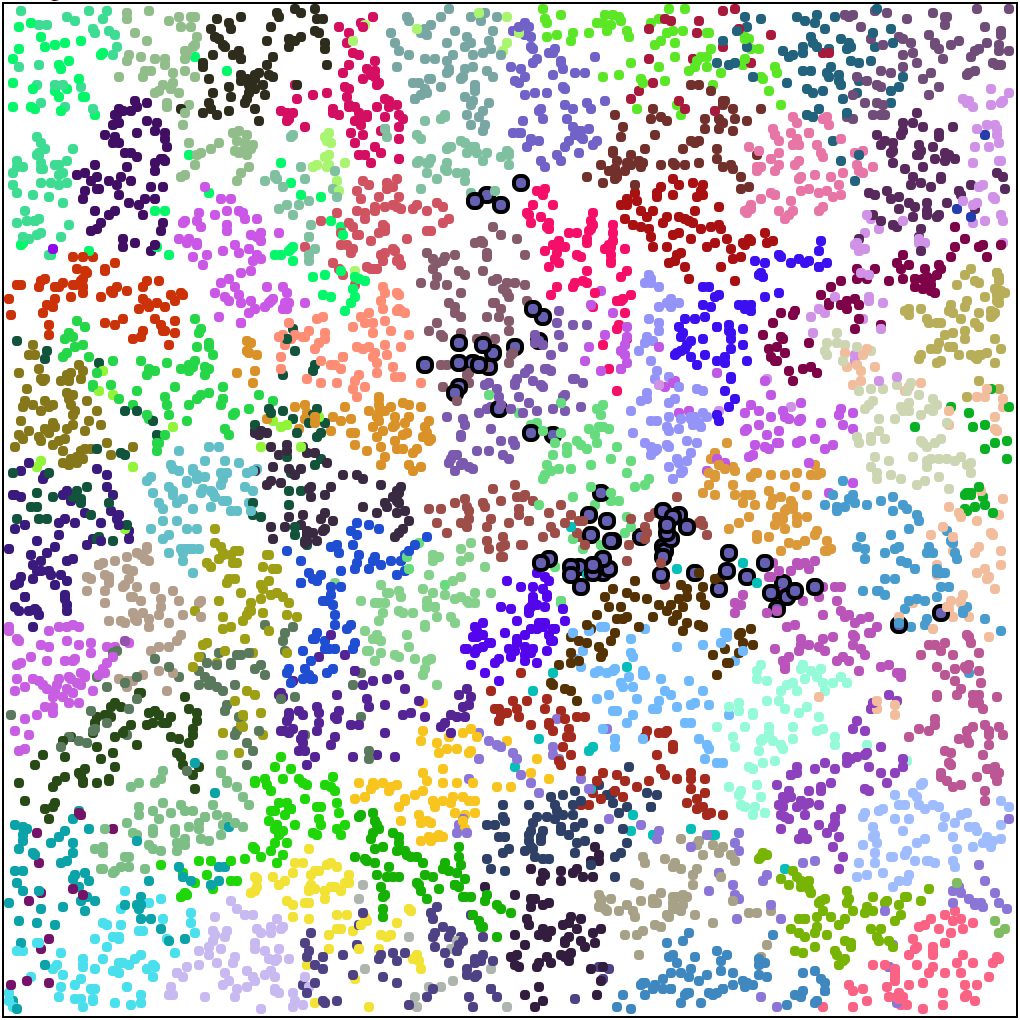
\includegraphics[scale=0.45]{Images/scenario3alt.png}
\caption{5000 nodes, $memberThresh=64$, $size=2000x2000$}
\label{fig:2000_64}
\end{figure}






%
%\begin{figure}
%\centering
%\begin{minipage}{.6\textwidth}
%	\center
%	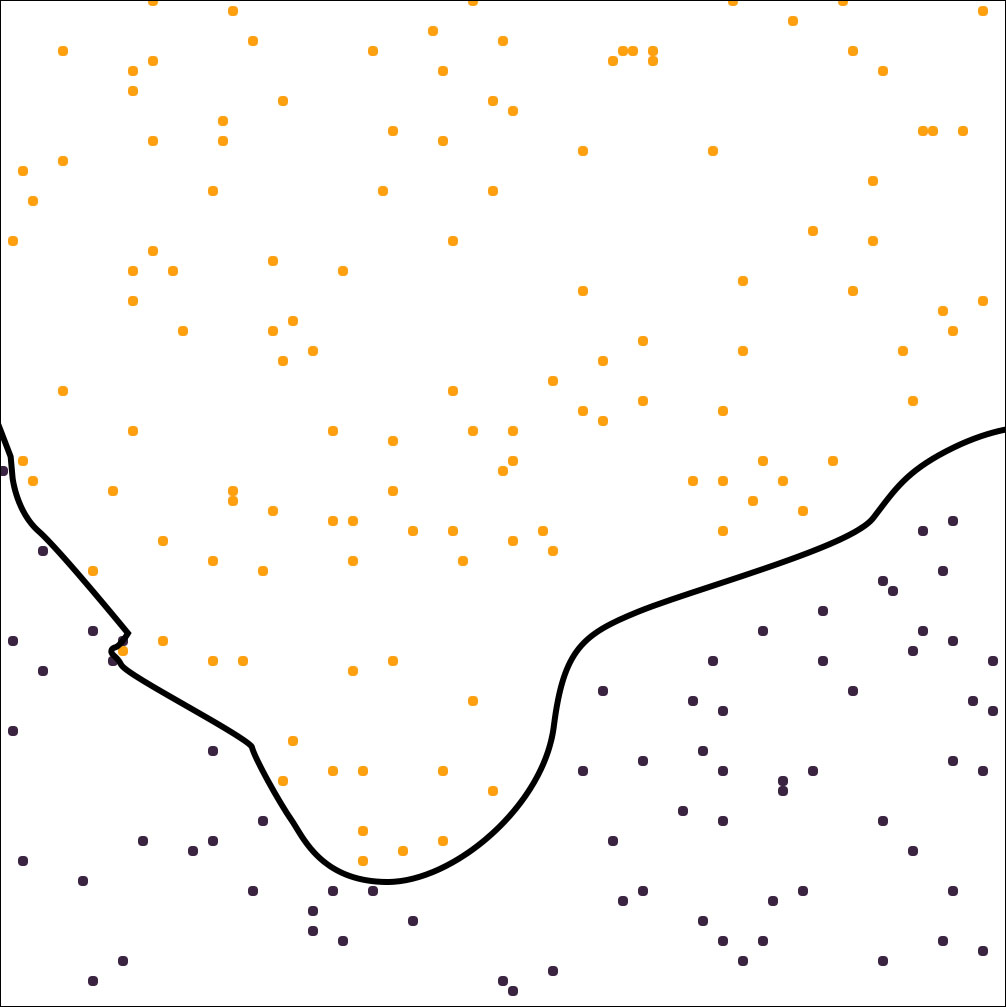
\includegraphics[width=0.9\linewidth]{Images/grouptest_1.jpg}
%	\captionof{figure}{\newline200 nodes, $memberThresh=128$}
%	\label{fig:200_128}
%\end{minipage}%
%\begin{minipage}{.6\textwidth}
%	\center
%	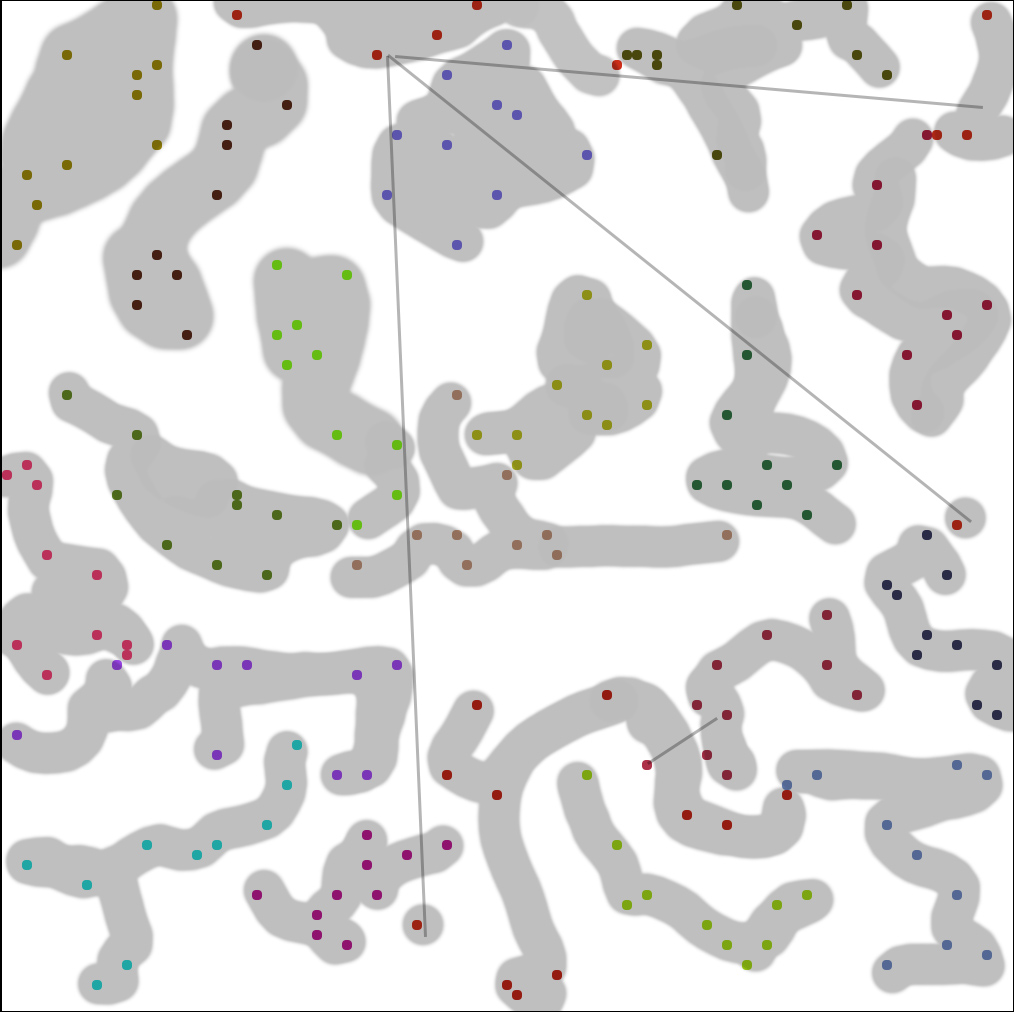
\includegraphics[width=0.9\linewidth]{Images/grouptest_2.jpg}
%	\captionof{figure}{Another figure}
%	\label{fig:test2}
%\end{minipage}
%\end{figure}




\section{Results}
By running the scripts that parses data from Wigle on populated areas, we should get an idea 
on how the algorithm performs in more realistic topologies. We will have a look at three
scenarios where the group allocation data is based on AP-data. 

Three suitable locations has been selected to perform the testing on Lillehammer (Norway)
a smaller city, Tynset (Norway) a less densely populated area, 
and Forks (Washington, United States). All tests were 
ran with a maximum group size of 128, and a $-dBi$ threshold of $-80$. 

\subsubsection{Lillehammer}
\begin{figure}
\center
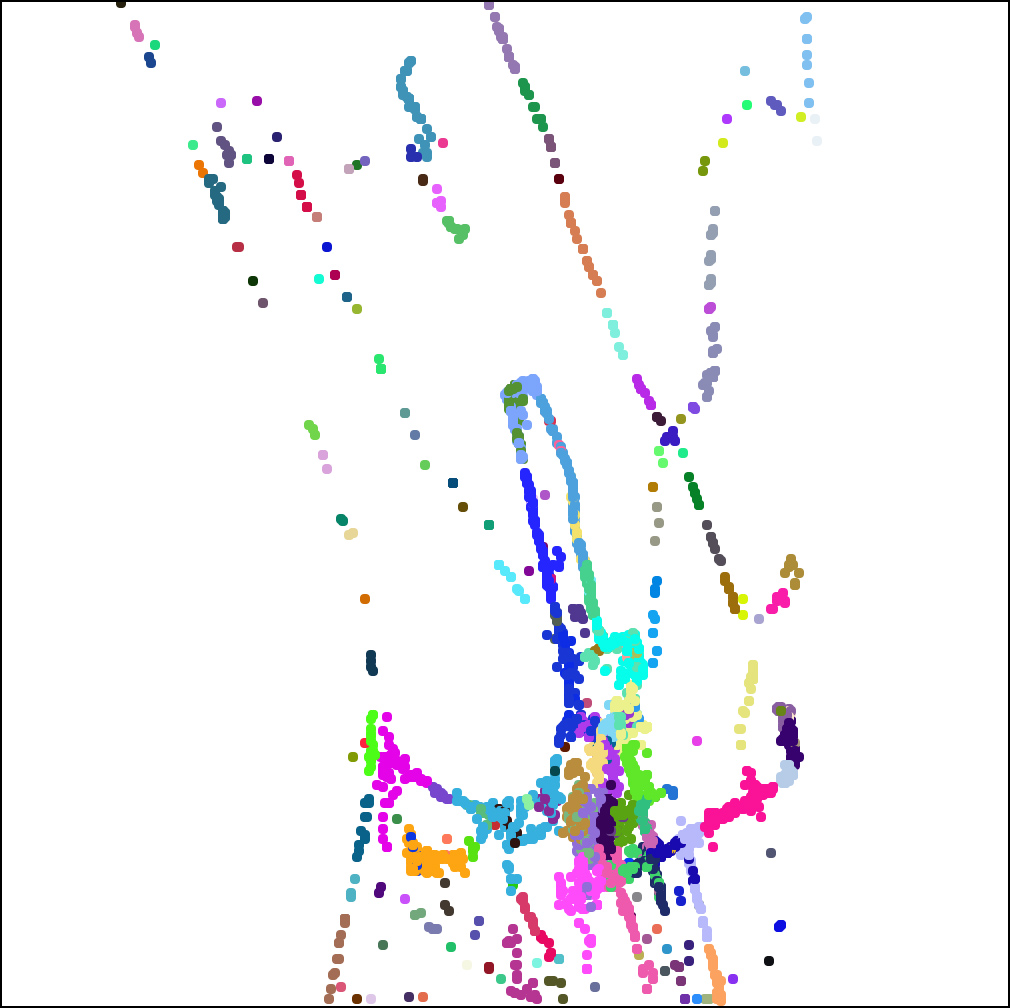
\includegraphics[scale=0.46]{Images/cities/lillehammer_groups.jpg}
\caption{Lillehammer}
\label{fig:lillehammer_topo}
\end{figure}

The computation results of Lillehammer can be seen in figure \ref{fig:lillehammer_topo}.
The topology is of medium density, consisting of 4990 APs, and is 2572 meters high 
and 8418 meters wide. From the tight clusters in the middle it is easy to make out the city centre.
We can clearly see different groups with different sizes. Some of the smallest groups
are highly likely so small because the distance to other nodes is too high for
the group to hear. In the denser areas they are occasionally very
entangeled, and it can be hard to make out the group borders.

Another thing to notice is that APs are nearly always placed in straight lines.
The straight lines are roads, and as Wigle collects data based on triangulation, the nodes
that is only seen once will get the position they are observed in, and not an actual
triangulated position. 
\subsubsection{Tynset}
The computation results of Tynset can be seen in figure \ref{fig:tynset_topo}. 
The topology consists of 726 APs, is 1670 meters high and  6720 meters wide. 
Unsurprisingly it resembles Lillehammer on a smaller scale.
Again we see
some very clearly defined groups, but in the city centre there are groups
which overlaps. We can also see nodes that are alone in their group,
because they are too far away from anyone else.
Much like Lillehammer, this topology is also strongly affected by the weak
triangulation of the APs, so most APs seems to be placed on top of a road. 

\begin{figure}
\center
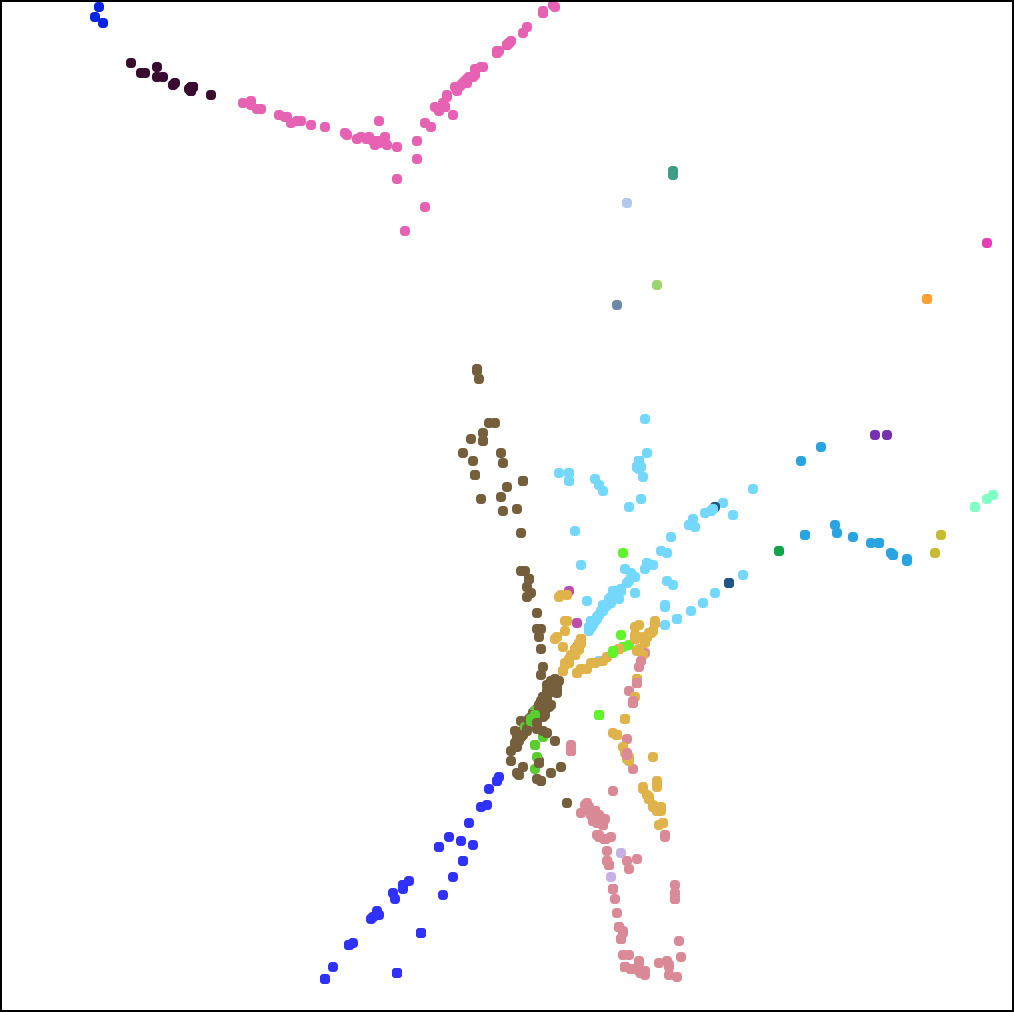
\includegraphics[scale=0.46]{Images/cities/tynset_groups.jpg}
\caption{Tynset}
\label{fig:tynset_topo}
\end{figure}

\subsubsection{Forks}

The computation results of Forks can be seen in figure \ref{fig:forks_topo}. 
The topology consists of 1715 nodes, and is 2122 meters high and 4495 meters wide. It
is important to include, because it is quite different from the other topologies and
represents a variation from the typical town and city structure of Norway.
The size of the groups are a little more uniform when comparing it to the others.
This can explained by the the smaller area the town is contained within. When a group
is not full, it will almost always hear someone that it can merge with.
We still have groups overlapping each other in the denser regions in Forks as well. 
What is worth noticing is that the APs are positioned more realistically as locations
of households. American towns looks more like a grid with roads in between households,
which makes triangulation easy and a lot more accurate. 

\begin{figure}
\center
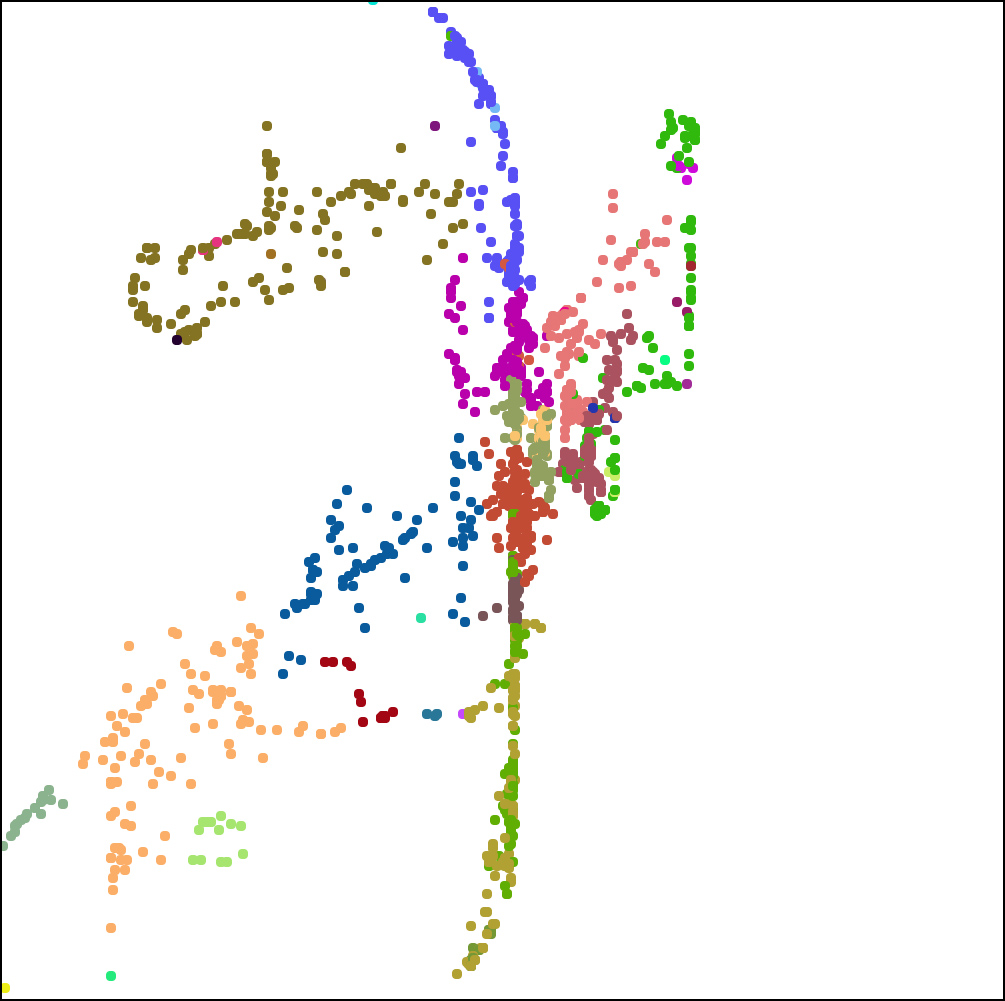
\includegraphics[scale=0.46]{Images/cities/forks_groups.jpg}
\caption{Forks}
\label{fig:forks_topo}
\end{figure}




